% Class Notes Template
\documentclass[12pt]{article}
\usepackage[margin=1in]{geometry} 
\usepackage[utf8]{inputenc}

% Packages
\usepackage[french, english]{babel}
\usepackage{amsmath, amsthm, amssymb ,amsfonts, graphics, tikz, float, enumerate, graphicx}
\usepackage{listings}
\usepackage{color} %red, green, blue, yellow, cyan, magenta, black, white
\definecolor{mygreen}{RGB}{28,172,0} % color values Red, Green, Blue
\definecolor{mylilas}{RGB}{170,55,241}

\lstset{language=Matlab,%
	%basicstyle=\color{red},
	breaklines=true,%
	morekeywords={matlab2tikz},
	keywordstyle=\color{blue},%
	morekeywords=[2]{1}, keywordstyle=[2]{\color{black}},
	identifierstyle=\color{black},%
	stringstyle=\color{mylilas},
	commentstyle=\color{mygreen},%
	showstringspaces=false,%without this there will be a symbol in the places where there is a space
	numbers=left,%
	numberstyle={\tiny \color{black}},% size of the numbers
	numbersep=9pt, % this defines how far the numbers are from the text
	emph=[1]{for,end,break},emphstyle=[1]\color{blue}, %some words to emphasise
	%emph=[2]{word1,word2}, emphstyle=[2]{style},    
}

% Title
\title{ECON 6140 - Problem Set \# 3}
\date{\today}
\author{Julien Manuel Neves}

% Use these for theorems, lemmas, proofs, etc.
\newtheorem{theorem}{Theorem}
\newtheorem{corollary}[theorem]{Corollary}
\newtheorem{lemma}[theorem]{Lemma}
\newtheorem{observation}[theorem]{Observation}
\newtheorem{proposition}[theorem]{Proposition}
\newtheorem{definition}[theorem]{Definition}
\newtheorem{claim}[theorem]{Claim}
\newtheorem{fact}[theorem]{Fact}
\newtheorem{assumption}[theorem]{Assumption}
\newtheorem{problem}[theorem]{Problem}
\newtheorem{set-up}[theorem]{Set-up}
\newtheorem{example}[theorem]{Example}
\newtheorem{remark}[theorem]{Remark}
\newtheorem{axiom}[theorem]{Axiom}

% Usefuls Macros
\newcommand{\field}[1]{\mathbb{#1}}
\newcommand{\N}{\field{N}} % natural numbers
\newcommand{\R}{\field{R}} % real numbers
\newcommand{\Z}{\field{Z}} % integers
\newcommand\F{\mathcal{F}}
\newcommand\B{\mathbb{B}}
\renewcommand{\Re}{\R} % reals
\newcommand{\Rn}[1]{\mathbb{R}^{#1}}
\newcommand{\1}{{\bf 1}} % vector of all 1's
\newcommand{\I}[1]{\mathbb{I}_{\left\{#1\right\}}} % indicator function
\newcommand{\La}{\mathscr{L}}
% \newcommand{\tends}{{\rightarrow}} % arrow for limits
% \newcommand{\ra}{{\rightarrow}} % abbreviation for right arrow
% \newcommand{\subjectto}{\mbox{\rm subject to}} % subject to

%% math operators
\DeclareMathOperator*{\argmin}{arg\,min}
\DeclareMathOperator*{\argmax}{arg\,max}
\DeclareMathOperator*{\maximize}{maximize}
\DeclareMathOperator*{\minimize}{minimize}
\DeclareMathOperator{\E}{\mathsf{E}} % expectation
\newcommand{\Ex}[1]{\E\left\{#1\right\}} % expectation with brackets
\DeclareMathOperator{\pr}{\mathsf{P}} % probability
\newcommand{\prob}[1]{\pr\left\{#1\right\}}
\DeclareMathOperator{\subjectto}{{s.t.\ }} % subject to
\newcommand{\norm}[1]{\left\|#1\right\|}
\newcommand{\card}[1]{\left|#1\right|}

% Extra stuff
\newcommand\seq[1]{\{ #1 \}}
\newcommand{\inp}[2]{\langle #1, #2 \rangle}

\newcommand{\inv}{^{-1}}

\newcommand{\pa}[1]{\left(#1\right)}
\newcommand{\bra}[1]{\left[#1\right]}
\newcommand{\cbra}[1]{\left\{ #1 \right\}}

\newcommand{\pfrac}[2]{\pa{\frac{#1}{#2}}}
\newcommand{\bfrac}[2]{\bra{\frac{#1}{#2}}}

\newcommand{\mat}[1]{\begin{matrix}#1\end{matrix}}
\newcommand{\pmat}[1]{\pa{\mat{#1}}}
\newcommand{\bmat}[1]{\bra{\mat{#1}}}

\begin{document}

\maketitle

\section*{Problem \#1}

	\begin{figure}[H]
		\centering
		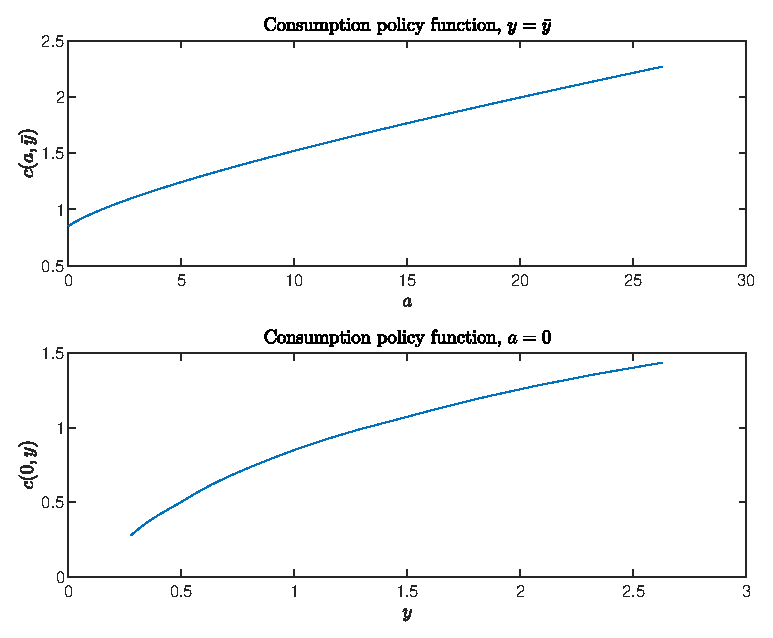
\includegraphics[width=0.7\linewidth]{fig1}
		\caption{Value function}
		\label{fig:fig1}
	\end{figure}
	\begin{figure}[H]
		\centering
		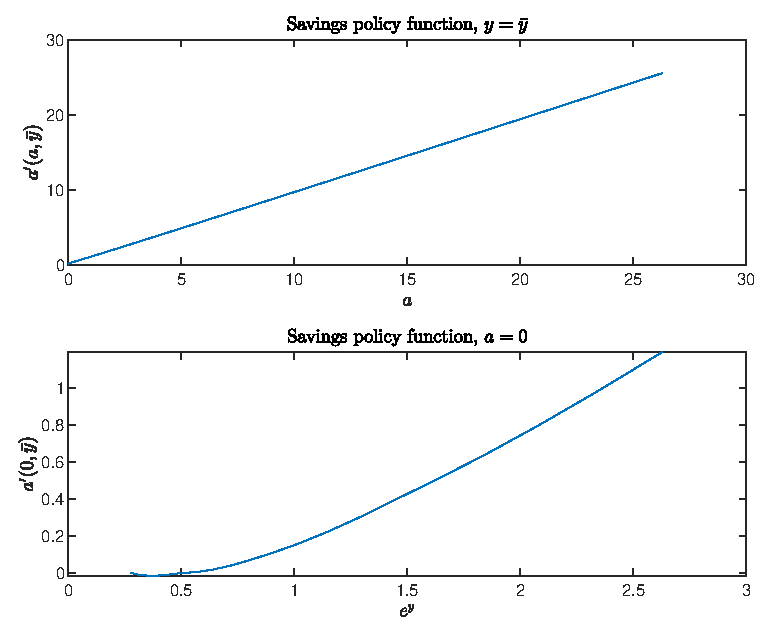
\includegraphics[width=0.7\linewidth]{fig2}
		\caption{Policy function}
		\label{fig:fig2}
	\end{figure}

	\begin{figure}[H]
		\centering
		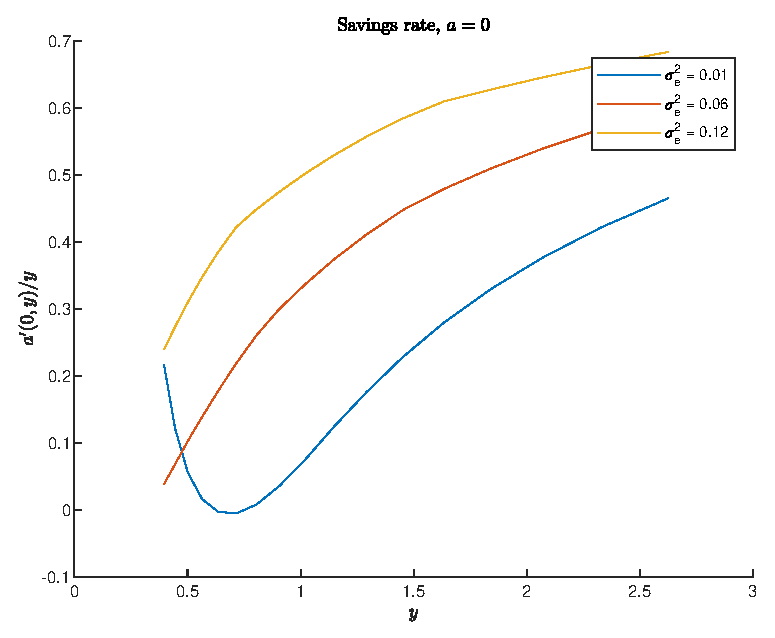
\includegraphics[width=0.7\linewidth]{fig3}
		\caption{Time path for consumption and capital}
		\label{fig:fig3}
	\end{figure}

	\begin{figure}[H]
		\centering
		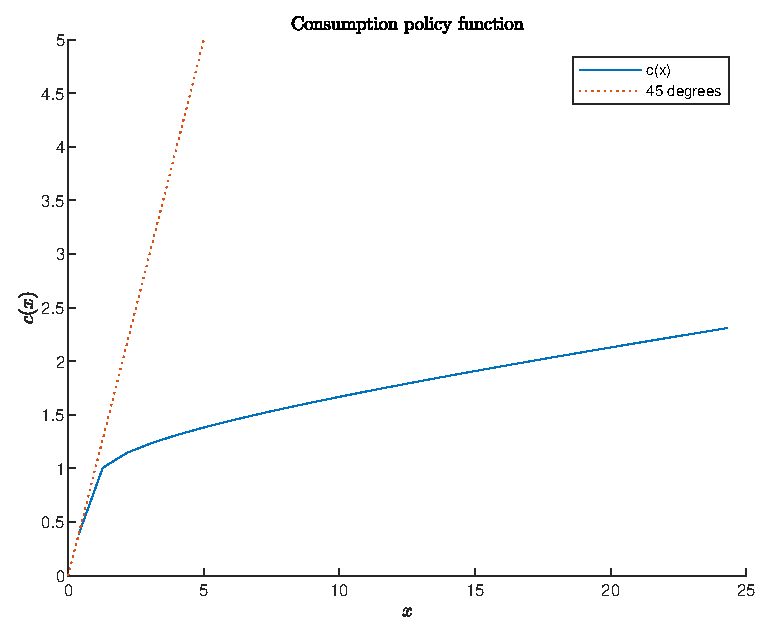
\includegraphics[width=0.7\linewidth]{fig4}
		\caption{Time path for consumption and capital}
		\label{fig:fig4}
	\end{figure}

	\begin{figure}[H]
		\centering
		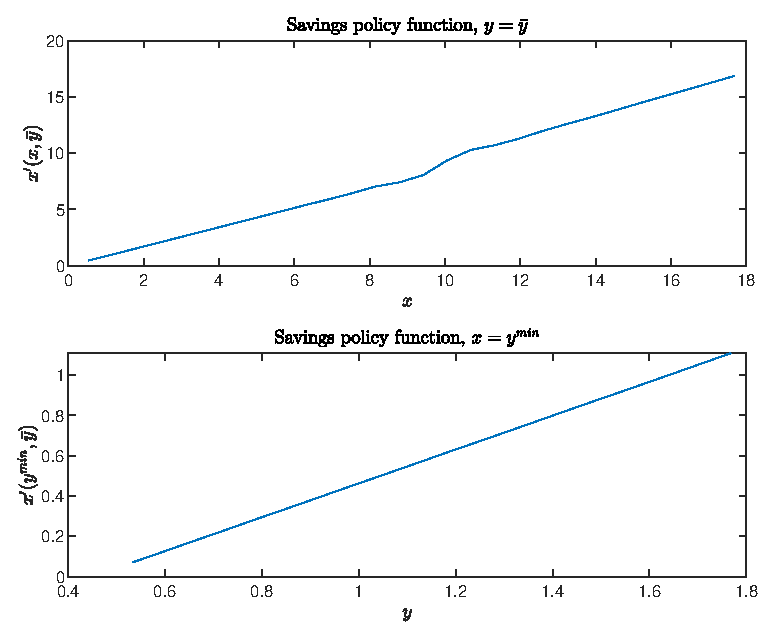
\includegraphics[width=0.7\linewidth]{fig5}
		\caption{Time path for consumption and capital}
		\label{fig:fig5}
	\end{figure}

\section*{Problem \#2}

\section*{Problem \#3}
	
\section*{Code}
\subsection{main.m}
\lstinputlisting[language=Matlab]{"main.m"}
\subsection{tauchen.m}
\lstinputlisting[language=Matlab]{"tauchen.m"}
\subsection{rouwenhorst.m}
\lstinputlisting[language=Matlab]{"rouwenhorst.m"}
\subsection{transition.m}
\lstinputlisting[language=Matlab]{"transition.m"}
\subsection{policy\_ip.m}
\lstinputlisting[language=Matlab]{"policy_ip.m"}
\subsection{solve\_ip.m}
\lstinputlisting[language=Matlab]{"solve_ip.m"}
\subsection{euler\_ip.m}
\lstinputlisting[language=Matlab]{"euler_ip.m"}
\subsection{policy\_ca.m}
\lstinputlisting[language=Matlab]{"policy_ca.m"}
\subsection{solve\_ca.m}
\lstinputlisting[language=Matlab]{"solve_ca.m"}
\subsection{euler\_ca.m}
\lstinputlisting[language=Matlab]{"euler_ca.m"}
\subsection{markovchain.m}
\lstinputlisting[language=Matlab]{"markovchain.m"}
\subsection{markovprob.m}
\lstinputlisting[language=Matlab]{"markovprob.m"}

\end{document}
